\chapter{Implementation}
\label{cha:implementierung}

\section{System Architecture}

The system architecture, depicted in figure \ref{fig:component_diagram}, integrates the behavior tree into the existing architecture. 
The already existing components are colored in gray, and the newly added components are colored in blue.
The new components and their functions are described in the following sections of this chapter.  

%This is done with the addition of the Decision Gate, that can selectively forward speed commands to the robot controller. The behavior tree's commands have a higher priority and disable the forwarding of the Navigation2 commands. 
%The behavior tree can access the sensor data when needed through the Data Backup component. The System Supervision component controls the health of all components, but the connections are not depicted in the component diagram for reasons of clarity and comprehensibility.

\begin{figure}[ht]
	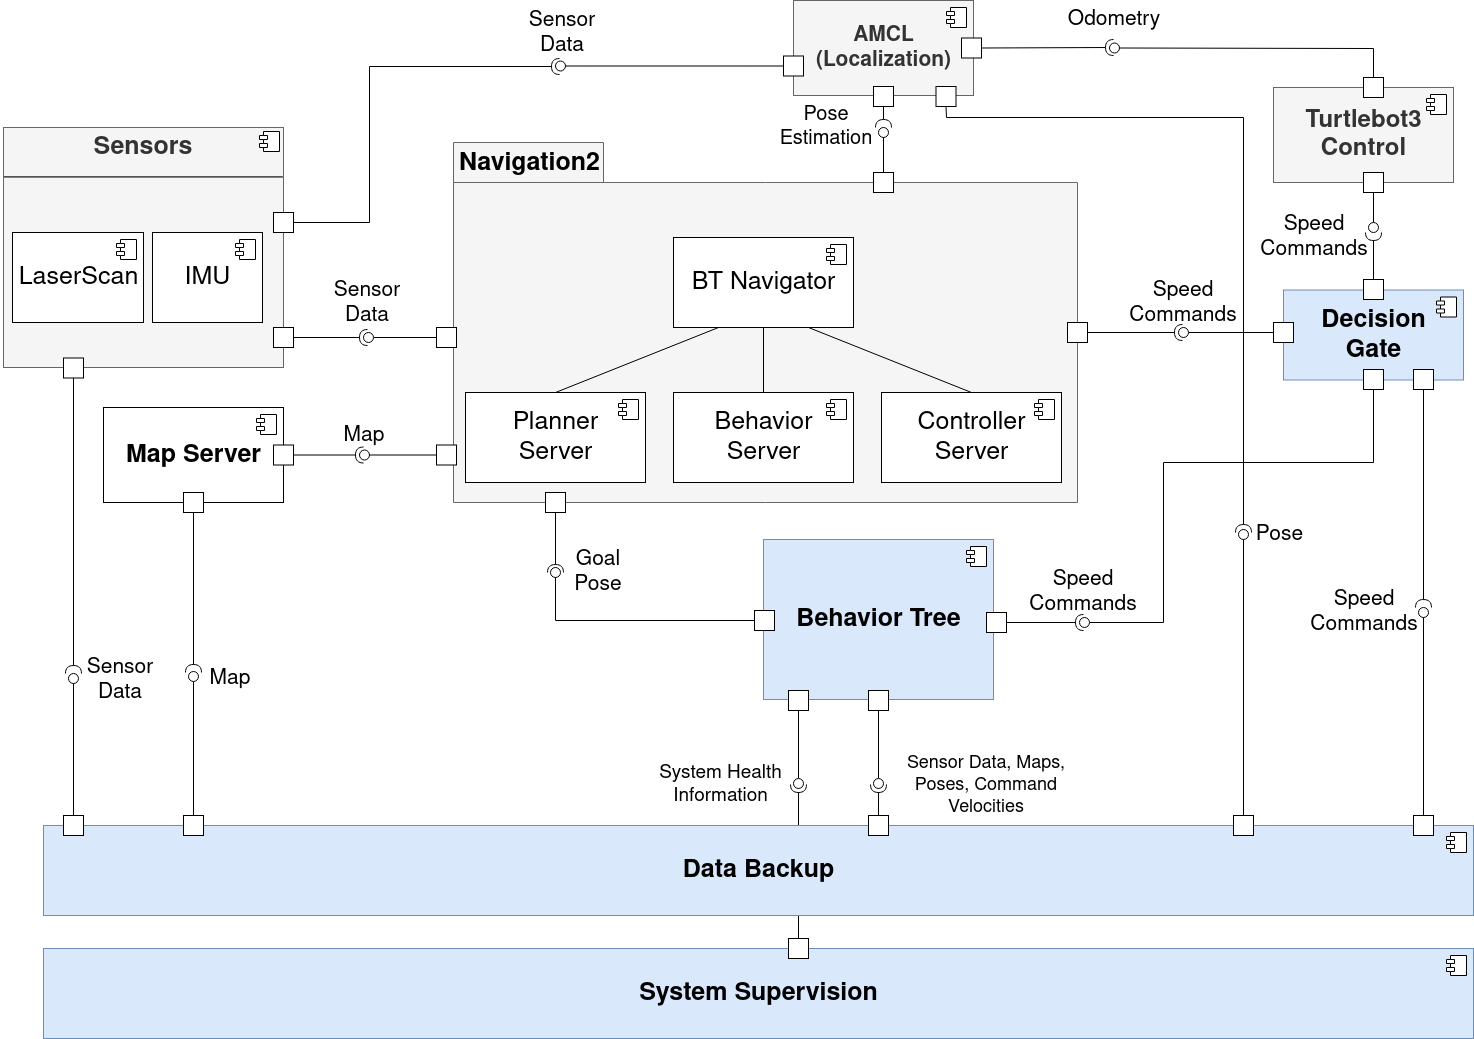
\includegraphics[width=1.00\textwidth]{images/component_diagram_bt.png}
	\caption{Component Diagram of System Architecture}
	\label{fig:component_diagram}
\end{figure}

\section{Data Backup}
The data backup component functions as a way to efficiently gather data from all system components and provide necessary data to the behavior tree when the planning process requires past data points. This component subscribes to all sensor data and saves the messages in a queue data structure. The most recent data gets pushed into the array, and if the array exceeds a specified length, the oldest data this data gets deleted from the array. There are two main reasons to limit the array size in this way. On the one side, the goal is to decrease the size of the message that gets sent to the BT to limit the network load, and on the other side, the BT often does not need to look back further than a few seconds to make a decision. This way, the computational load, and the network load are decreased.
\paragraph*{}

The BT can access the saved data by sending a service call to one of the provided services by this component. Service calls in ROS2 are executed with high priority and are done quickly. However, it adds steps to the algorithm instead of just saving the data directly in the behavior tree. The reason for outsourcing the data backup to another component is that the ROS node needs an executor which constantly spins the node. The spinning action checks the network to see if there is any work for the node. Work, in this context, means that if one of the subscribed topics receives a message, the node has to execute one of its callback functions associated with that subscription. This spinning has to be done in regular intervals. Otherwise, the node might miss incoming messages from subscribed topics. The way to do the spinning is to have the node constantly spun in one thread. Having a constant spinning node would completely block the behavior tree's execution. If one tries to spin a node once when a node gets ticked in the BT, the problem of missing messages will become relevant because the BT might need longer than expected to return to a node to tick it. That way, the BT node responsible for saving all the relevant data can not guarantee that it has picked up on all the messages between spins. The synchronous nature of the ROS executor spinning the nodes is why the data backup is not stored within the BT. 
The saved data inside this component with the corresponding lookback time is listed in table \ref{tab:data_backup_types}. 

\begin{center}
\begin{table}[ht]
	\caption{Types of saved data}
	\label{tab:data_backup_types}
	\begin{tabular}{ | m{0.2\textwidth} | m{0.25\textwidth}| m{0.25\textwidth} | m{0.2\textwidth} |} 
  	\hline
  	\textbf{Name} & \textbf{Type} & \textbf{Lookback Time} \\ 
  	\hline
  	Lidar & Laserscan & 3 seconds \\
  	\hline
  	Poses & Pose with Covariance & 2 seconds\\ 
  	\hline
  	Map & Occupancy Grid & Only saved last one \\ 
  	\hline
  	Collision Pose & Pose with Covariance & Only last one \\
  	\hline
  	Command Velocities & Twist & 2 seconds\\
  	\hline  	
  	Global Costmap & Occupancy Grid & Only last one \\
  	\hline
	\end{tabular}
\end{table}
\end{center}


\section{Command Velocity Decision Gate}

This component is responsible for modifying or blocking the Velocity Commands from Nav2. The component receives messages from Navigation2 on the "/cmd$\_$vel$\_$nav" topic and the "/cmd$\_$vel$\_$bt" topic from the behavior tree. This component publishes the received messages on the actual topic "/cmd$\_$vel" which is subscribed by the robot controller. 
The BT can modify the Decision Gate parameters to either disregard incoming messages of Nav2 entirely or to modify them. The modification is helpful when the situation demands the robot to slow down. 
If the Decision Gate receives messages from Nav2 and the BT, it will prioritize the BT. This situation should theoretically never occur as the BT will set the parameters for the Decision Gate accordingly and cancel the current Navigation Goal before publishing commands on its own. It is implemented as an additional safety measure in case the cancellation of the goal is not possible if Navigation2 is not responsive to the cancellation command. 

\section{Behavior Tree Structure}

A simplified behavior tree only depicting the top-level behavior control fallback nodes is shown in figure \ref{fig:top_level_bt}. The tree receives the initial tick signal from the root in an infinite loop. 

\begin{figure}[ht]
	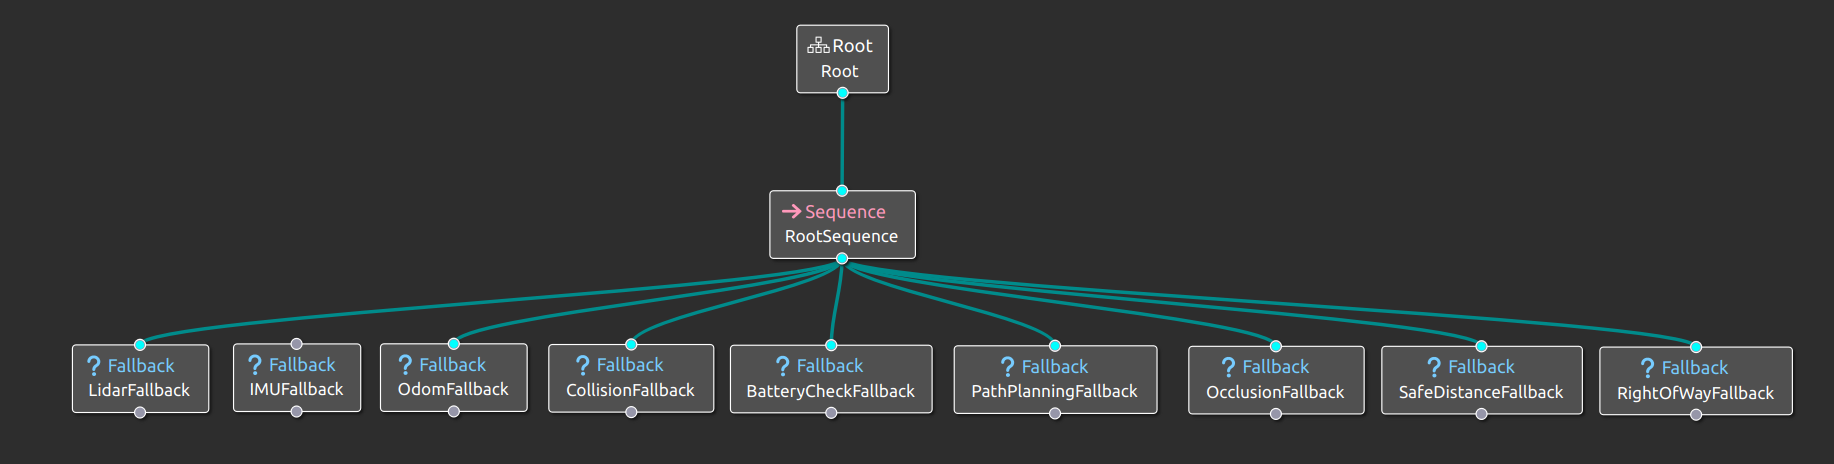
\includegraphics[width=1.0\textwidth]{images/simplified_bt.png}
	\caption{Top Level Behavior Tree Structure}
	\label{fig:top_level_bt}
\end{figure}

The root control node is a sequence node. The root node is a simple sequence because the whole system must function with increasing complexity in the tree's later parts (on the right side). The complex behaviors require that all previous components and conditions work as they should. The root sequence will not allow the execution of higher-level behaviors if the system detects problems on more fundamental levels. The root sequence is the first step for increasing the system's robustness to combat competing reactive and deliberative behaviors that could endanger the robot's safety and other actors in its environment. 

\subsection{BT System Supervision}

The design pattern of the system supervisor is an "Watchdog" pattern. This pattern is depicted in figure \ref{fig:watchdog_pattern}. The pattern is used to monitor a system from the outside and directly take corrective measures when problems are detected. 

\begin{figure}[ht]
	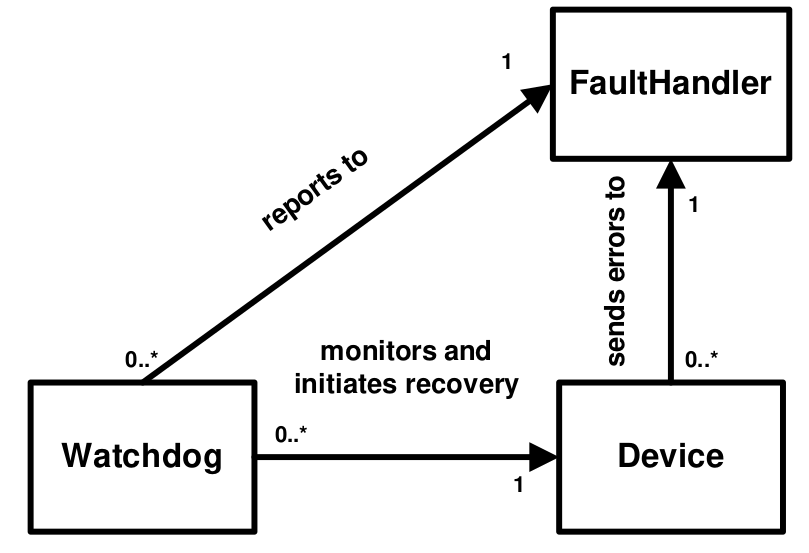
\includegraphics[width=0.4\textwidth]{images/watchdog_pattern.png}
	\caption{Examiner pattern for the system supervisor component \cite{konrad2003defining}}
	\label{fig:watchdog_pattern}
\end{figure}

The system supervisor component is partly outsourced into a component outside of the BT's thread for the same reasons as the sensor backup component discussed in the previous section. The synchronous executor would stop the execution of the whole behavior tree, which is why the component needs to be moved inside of a new thread. The system supervisor, also called the execution checker, is receiving messages from nodes not implemented as ROS2 lifecycle nodes. If a node stops sending messages or responding completely, the external execution checker can inform the BT via a provided service of a problem with the node. ROS2 lifecycle nodes provide information about their health via an FSM implementation inside the node. The current node state can be requested via a service call. However, the node's output needs to be checked, too, because it might be that the FSM inside of the node did not pick up on an error and failed to change the internal lifecycle state. 
The system supervision is constantly checking the system's health. The BT is using service calls to get the health information about the components checked inside Condition Nodes. 
The components get checked by the BT inside of a Fallback. If the condition for the execution is met, the Condition Node returns "Success", and the fallback would exit to move on to the next fallback and execution condition check (see fig. \ref{lidar_fallback}). If the execution checker detects a node failure, a sequence to react to the sensor failure is executed in which the robot slows down to a minimum and tries to restart the sensor. Should the restart fail twice, the robot will not be able to navigate safely anymore and will come to a complete stop. This behavior pattern is realized for the lidar, the IMU, and the wheel odometry. 
\begin{center}
\begin{figure}[ht]
	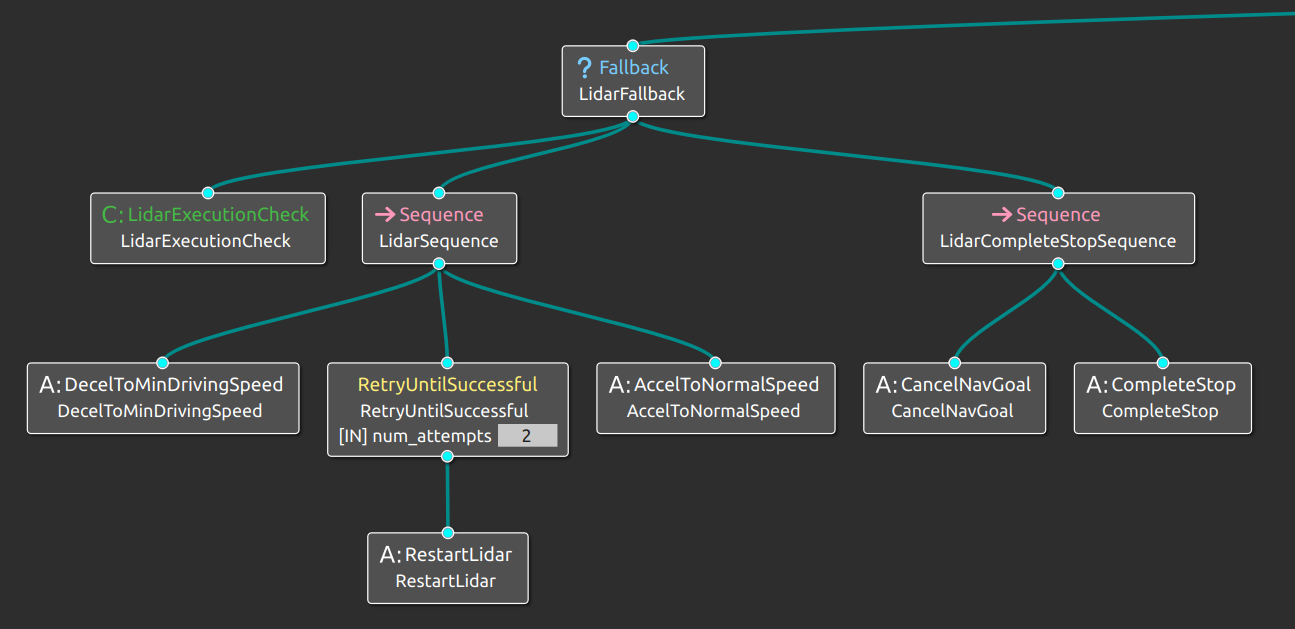
\includegraphics[width=1.0\textwidth]{images/sensor_fallback.png}
	\caption{Lidar Fallback}
	\label{fig:lidar_fallback}
\end{figure}
\end{center}


The timeout period for the execution checker to declare a node failed after receiving no message is set at one second. 
After that period, the goal is to enable the robot to continue progressing towards the goal. However, if the system can not restart the sensor in a short time after failure, the robot has to come to a stop as a sensor failure is a severe function loss for the robot.

\subsection{BT Advanced Behaviors}
After the BT has checked for sensor failures and can guarantee that the environment representation is accurate, the system can check for more complicated scenarios to improve autonomy. The implemented behaviors are outlined in this section. 


\subsubsection{Collision Behavior}

One of the biggest problems mentioned in chapter 3.1 is the inability to react to collisions. The collision can happen due to inadequate sensory coverage for detecting obstacles or general sensor inadequacy, which can not detect obstacles because of their shape or surface material. Collisions would be improbable with many sensors covering all angles and heights and computer vision capabilities to detect obstacles. However, even if the robot could detect all obstacles, it would still be vulnerable to outside perturbations, e.g., other robots driving into it or humans accidentally touching the robot. 
In order to combat this weakness, the robot must be able to detect that a collision occurred, get out of the collision state, update the map and reset all costmaps to generate a new path to the original goal. 

\begin{figure}[ht]
	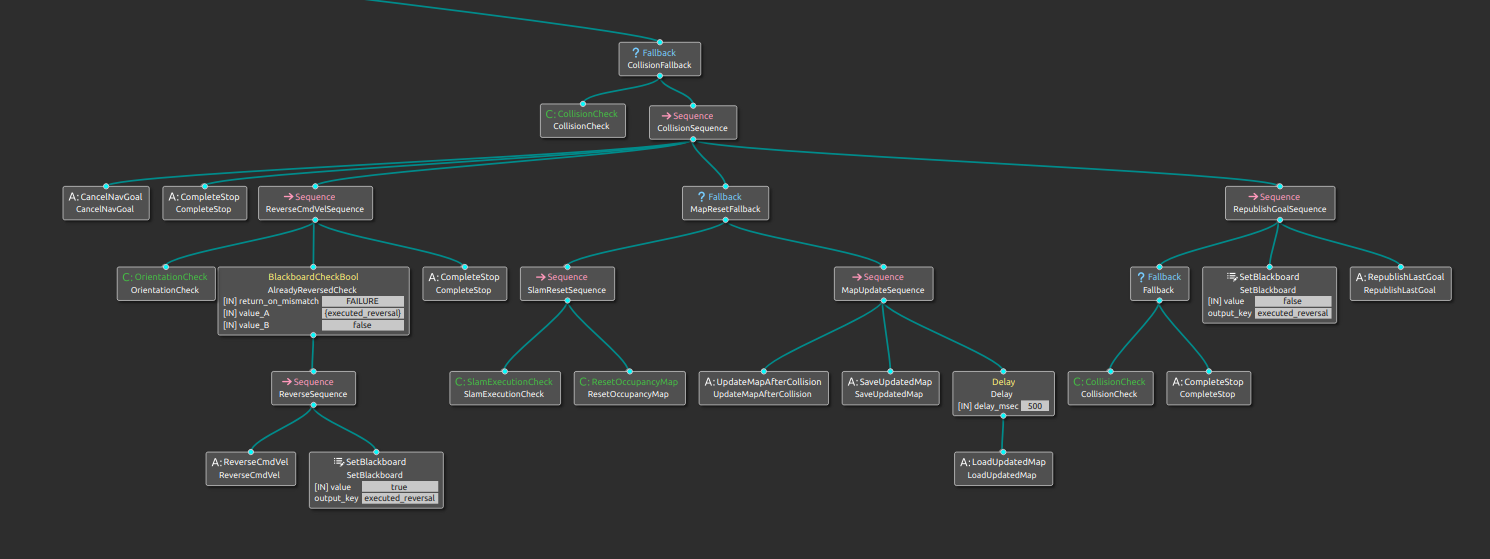
\includegraphics[width=1.0\textwidth]{images/collision_fallback.png}
	\caption{Collision Fallback Behavior}
	\label{fig:collision_fallback}
\end{figure}

\subparagraph*{}
The collision checker uses a simulated sensor to detect collisions. On a real robot, the collision checker can use an IMU-based collision detection, but this has not been implemented in this behavior tree due to the time constraints of this thesis. The collision checker is integrated into the system supervisor, and the BT makes service calls to the execution checker to get the collision state of the robot periodically. 
The child nodes of the collision sequence use the sensor data backup. 
To get out of the collision state, the BT requests the last saved command velocities from the data backup component and modifies them to reverse with minimum speed the same way the robot got into the collision. The reversing action takes longer than the two seconds as the commands get published with more extended time intervals between them to adjust the driven distance to be the same as the navigation commands. An additional check is implemented before the reversing to ensure the robot only reverses once. Otherwise, the robot would drive back and forth as the data backup service would provide the BT with the commands from the last reversing action. 

%The modification is done in the following manner
%
%\textit{Formula for determining execution time}
\subparagraph*{}
Regarding the map reset, it has to be determined if a new map is being created with a SLAM method or if the map server provided a previously saved map. In the case of the running SLAM, the recent updates to the map must be discarded, and a previous map version before the collision has to be re-utilized. When the map server component from Nav2 provides a static map, the map needs to be updated with a new obstacle at the point of collision and republished by the map server. 
The activity of the "MapUpdateAfterCollision" action node is depicted in figure \ref{fig:activity_diagram_collision}. The collision point is estimated by the robot's pose, which refers to the robot base link and the robot footprint. It is assumed that the collision point was right in front of the robot because the local planner favors forward drive kinematics and probably is driving forwards when a collision occurs. The simulated bumper sensor can provide more nuanced information about the point of contact, but this functionality can not be achieved on a real robot with IMU-based collision detection. Hence the obstacle position is simplified to always be in front of the robot. 
%The collision position is calculated with 
%
%\textit{Formula here}

A 25 by 25 cm square with 100 percent occupation at the collision point is added to the current map and then saved to be reloaded by the map server. 
%as depicted in figure xx. 
% add the 

\subparagraph*{}
The original goal is then republished to replan the global path on the updated map. A more detailed view of the whole behavior is depicted in figure \ref{fig:activity_diagram_collision}.

\begin{figure}[ht]
	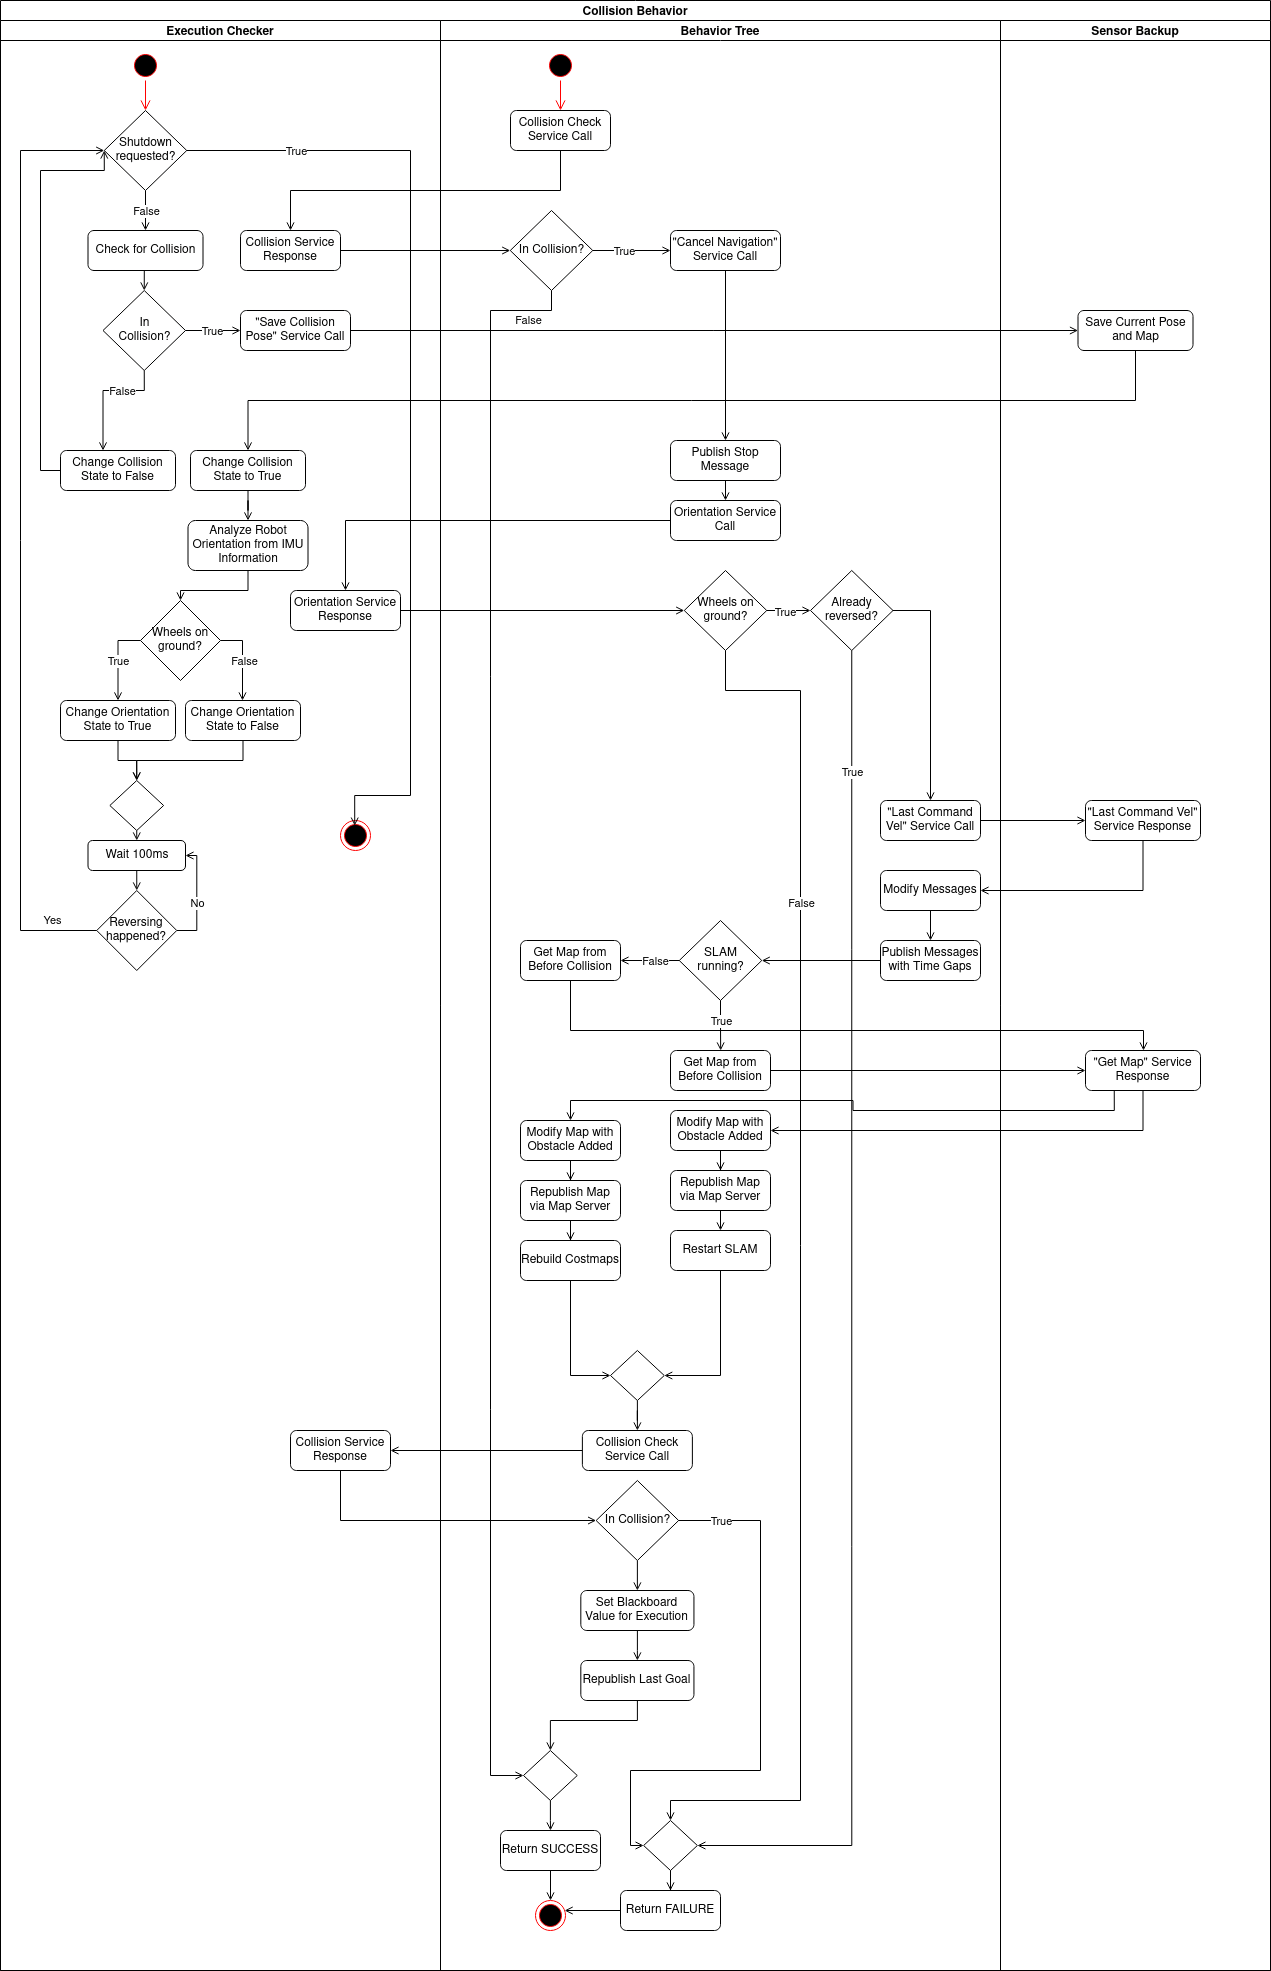
\includegraphics[width=0.95\textwidth]{images/activity_diagram_collision.png}
	\caption{Activity Diagram for the Collision Behavior}
	\label{fig:activity_diagram_collision}
\end{figure}

This way, obstacles lower than the lidar scan height can be detected. With this behavior, the robot should be able to eventually navigate around transparent obstacles that do not reflect the laser. Glass doors are known to cause issues for robots based only on lidars. 

\subsubsection{Battery Behavior}

The battery behavior has the goal of monitoring the robot's battery and has to decide if the robot should navigate to a new goal location or not. The decision is based on the current battery charge and the estimated consumption of energy to reach the new goal. The robot should not begin the navigation process if it is probable that the remaining charge will not suffice for the driving. Figure \ref{fig:battery_fallback} depicts the behavior tree fallback.

\begin{center}
\begin{figure}[ht]
	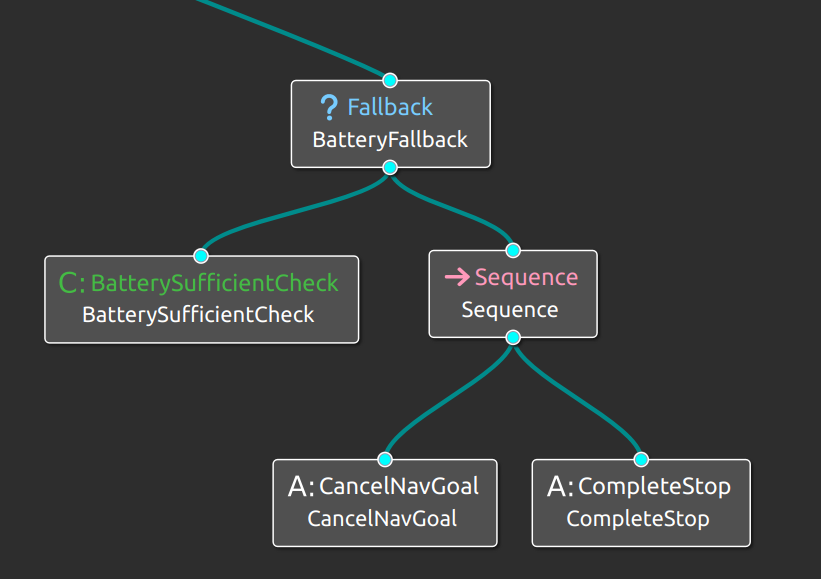
\includegraphics[width=0.5\textwidth]{images/battery_fallback.png}
	\caption{Battery Fallback Behavior}
	\label{fig:battery_fallback}
\end{figure}
\end{center}

The robot has to consider the idle consumption and the energy to drive the motors. With this information, a linear function for energy expenditure was created to predict battery usage depending on the path length. An additional safety factor was added to the energy estimation function to consider the scenario in which the robot must reroute and drive a longer route or stop for a moment. The safety factor was included to increase the behavior's robustness and cover more scenarios.
%The resulting function can be described as: 
%
%\textit{Formel here}
\subparagraph*{}

The average values for idle and driving consumption on a real robot could be experimentally determined. For the simulated turtlebot, a simulated battery package was created, which updates the battery charge every second. The battery package subscribes to the command velocity topic and decreases the battery charge for every message received. The battery package was created because the behavior for this scenario needs to be tested, and Gazebo does not offer this function. The consumption rates are not close to reality but are chosen to allow the rapid testing of the behavior.
The battery package provides a service to get the battery charge and the values for the assumed consumption rates while idle and driving (compare \ref{tab:custom_interfaces}. The BT node "IsBatterySufficientCheck" calls the service to compare the current battery to the calculated consumption. The battery behavior fallback will cancel the navigation goal if the robot can not reach the given goal with the remaining charge.

\subsubsection{Path Planning Behavior}

With this behavior, a way to make the global planner more flexible was implemented. 
The execution checker component monitors the health of the Nav2 global planner. Additionally, the behavior tree analyses the global planner's output. If the latter condition fails, the given navigation goal is not reachable by the planning algorithm. By shifting the goal to a nearby alternative goal, the robot tries to navigate, although the original goal is not reachable. If the location is still unreachable, the goal gets moved further away from the original. The routine repeats up to ten times, leading to a maximum distance to the original goal of up to one meter. 
The goal gets moved on a straight vector towards the robot. Other strategies for finding alternative goals were not implemented in this behavior. Figure \ref{fig:global_planning_fallback} depicts the behavior tree fallback for the behavior.

\begin{center}
	\begin{figure}[ht]
	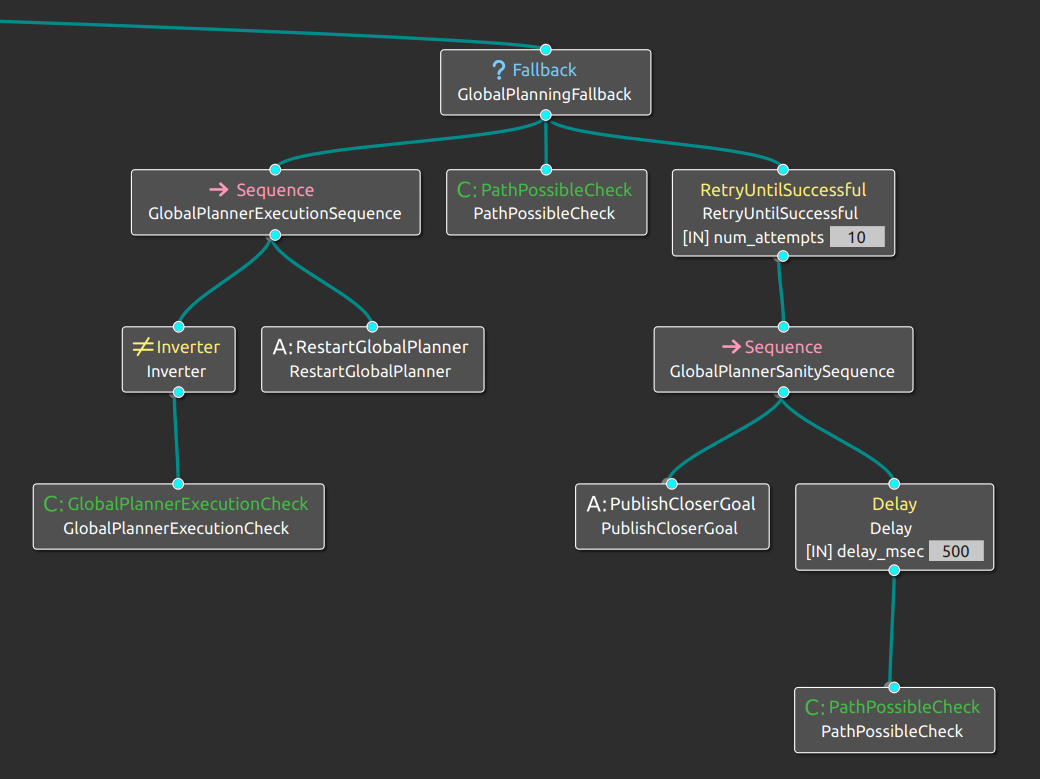
\includegraphics[width=0.7\textwidth]{images/global_planning_fallback.png}
	\caption{Path Planning Fallback Behavior}
	\label{fig:global_planning_fallback}
	\end{figure}
\end{center}

\section{System Support Tools}
\subsection{Gazebo Sensor Drivers}
%\label{sec:gazebo_driver}
For testing purposes, the simulated sensor data is not published directly on the actual topic by Gazebo. An intermediary node is used, which subscribes to the Gazebo topic and republishes the information on the original topic. The failure of a sensor can be simulated this way by stopping the execution of the intermediary node. Figure \ref{fig:rqt_graph} shows the RQT graph, which depicts the ROS nodes and their subscribed/published topics. 

\begin{center}
\begin{figure}[ht]
	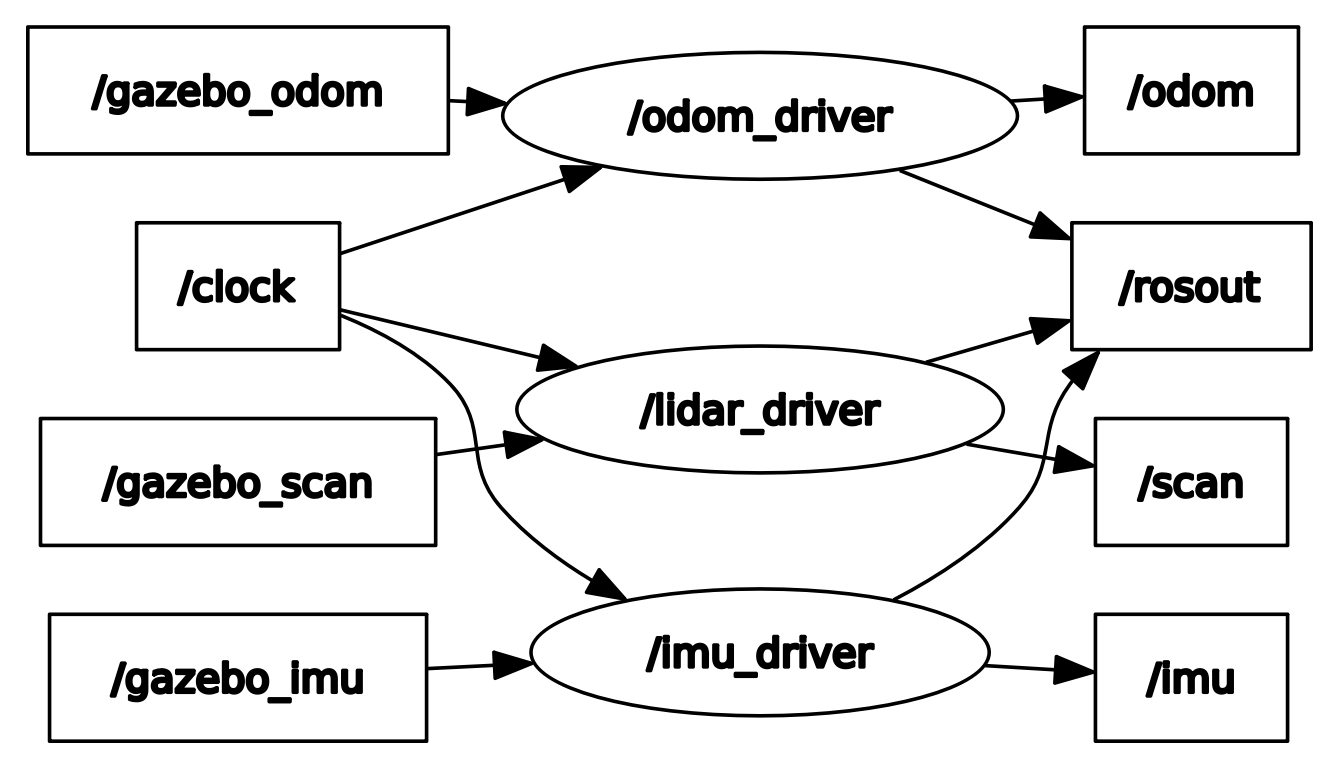
\includegraphics[width=0.75\textwidth]{images/rqt_graph_sensor_drivers.png}
	\caption{Graph for the Sensor Driver nodes and topics}
	\label{fig:rqt_graph}
\end{figure}
\end{center}

\subsection{Custom ROS Interfaces}

Because of the necessity to have ROS nodes spinning outside of the BT thread, as discussed in 4.4.1, additional interfaces needed to be created in order to receive information through service calls. The created service types are listed in table \ref{tab:custom_interfaces}. All service definitions are created in a dedicated package named "bt$\_$msgs". 

\begin{table}[ht]
	\caption{Implemented Custom Services}
	\label{tab:custom_interfaces}
	\begin{tabular}{ | m{0.2\textwidth} | m{0.33\textwidth}| m{0.33\textwidth} | m{0.2\textwidth} |} 
  	\hline
  	\textbf{Name} & \textbf{Request} & \textbf{Response} \\ 
  	\hline
  	GetCharge & Empty & float charge, float idle$\_$decrease$\_$per$\_$sec, float drive$\_$decrease$\_$per$\_$sec \\
  	\hline
  	GetDistance & Empty & float distance$\_$in$\_$meter\\ 
  	\hline
  	GetLastGoal & Empty & geometry$\_$msgs/Pose last$\_$goal$\_$pose \\ 
  	\hline
  	GetLastMap & Empty & nav$\_$msgs/OccupancyGrid map \\
  	\hline
  	GetTwistArray & Empty & geometry$\_$msgs/Twist[] cmd$\_$vel$\_$array\\
  	\hline  	
  	PubCmdVel & geometry$\_$msgs/Twist cmd$\_$vel, float time$\_$in$\_$seconds & bool success \\
  	\hline
  	SendUpdatedMap & nav$\_$msgs/OccupancyGrid updated$\_$map & Empty \\
  	\hline
	\end{tabular}
\end{table}
